\documentclass[pageno]{jpaper}

%replace XXX with the submission number you are given from the ISCA submission site.
\newcommand{\iscasubmissionnumber}{XXX}

\usepackage[normalem]{ulem}

\begin{document}

\title{
Basic-block Architecture}

\date{}
\maketitle

%\thispagestyle{empty}

%%%%%%% ABSTRACT %%%%%%%
\begin{abstract}

The main factors contributing to the bulk of energy consumption in modern
out-of-order processors are the speculative logic units, dynamic instruction
scheduling modules, and on-chip data movement.  This work significantly reduces
these energy overheads via introducing compiler-generated techniques that enable
near in-order energy consumption while maintaining near out-of-order computation
performance. Specifically, we introduce the notion of coarse-grain program
execution; in this model, program basic-blocks are speculatively run
out-of-order while instructions within each basic-block run in-order.
Basic-block execution closes up to 90\% of the energy gap and 78\% of the
performance gap between in-order and out-of-order.

\end{abstract}

%%%%%%% BODY %%%%%%%
\section{Introduction} 
\label{sec:intro}

As described by~\cite{mcfarlin2013discerning}, the exceptionally high
performance of out-of-order (OoO) processors is fundamentally due to two key
attributes: dynamism and speculation.  Lack of either feature can significantly
impact its performance. 

The key sources of energy consumption in OoO processors is data-movement and __
(back this up).

BBS is a hardware-software scheduling hybrid technique that enables significant
energy savings in the processor while maintaining near the same level of
performance as the out-of-order processor. This hybrid model is constructed
based on the notion of coarse-grain out-of-order execution where the term
coarse-grain refers to the ability of the processor to execute groups of
instructions out of program order. Each group executes its instructions in order
while multiple such groups execute their instructions out of program order.

%\section{Basicblock Scheduling}
\label{sec:bb_sch}



\section{Microarchitecture}
\label{sec:arch}

Coarse grain execution exposes energy saving opportunities in most pipeline
stages. In this section we discuss the flow of basicblocks through different
pipeline stages and elaborate on how energy is saved in each stage.

Below, we discuss the various architectural components of this architecture.
Figure XX illustrates the processor stages in detail.

\subsection{Basicblock Structure}
\label{sec:bb_struct}

What: discuss bb binary structure including its header contents: branch address.
Also explain the hardware support structure to hold register renamed values for
each global operands (both rad and write). it also contains the BB SN.

Why: to show how we save energy by BP lookup and energy efficient renaming
(renaming buffer is tiny, and cheap to access for both ready-check and wake-up
 logic). energy efficient and more high performance branch prediction.

(make a note that bb header for holding register operands is a CAM array)

% Basicblock boundaries are explicitly annotated by the compiler in the program
% binary through special header instructions (H) that contain certain key
% information about the BB; H instructions hold the BB branch instruction address
% (unless the BB is terminated without a branch or jump operation), global read
% registers, and global write registers used in the BB. Figure XX illustrates the
% organization of each H instruction.
% 
% Contrary to existing processors where the branch-prediction unit (BPU) is looked
% up on every fetch group regardless of the type of instructions in the fetch
% group, BB looks up the branch predictor only through H instructions. Immediately
% after the decode stage, H instructions feed the address of the upcoming branch
% instruction to BPU to find the PC of the next basicblock. This approach
% significantly reduces the traffic to BPU reducing mis-predictions due to
% aliasing and lookup energy consumed unnecessarily by non-branch instructions.
% 
% Global write registers used by instructions in the basicblock are incorporated
% in H so that ?.
% 
% Global read registers used by instructions in the basicblock are incorporated
% in H so that the wake-up logic would simply ?.
% 
% Discussion on instruction overhead (for i-cache) of adding H instructions to the ISA.

\subsection{CPU Frontend}
\label{sec:cpu_frontend}

discussion of register renaming and branch prediction lookup and update models.

% The processor frontend consists of the branch-prediction, fetch, decode, and
% register rename stages. Branch prediction only looks up H instructions. Fetch
% and decode stages are designed similar to existing architectures with
% configurable withs of 2, 4, 8. Contrary to the OoO model where register renaming
% happens in dispatch stage, here register renaming is done right after decode
% (explain why).  The register rename unit is only accessed by H instructions.
% Local registers do not access the register rename unit.
% 
% Given the smaller utility of register renaming, this processor can use a
% smaller set of physical registers (less area and energy per access).

\subsection{CPU Backend}
\label{sec:cpu_backend}

The backend consists of several basicblock window buffers used to store
basicblock operations and the meta-data associated with each BB, local registers
for each basicblock, a global register file, execution units, basicblock reorder
buffer (BBROB), a load-store queue model, and the wake-up logic.

%\subsubsection{Basicblock Window}
\label{sec:bb_window}

\textbf{BB Windows} are FIFO buffers used to store up to 16 outstanding
instructions.  Instructions in a BB Window execute in-order. In
Figure~\ref{fig:bb_arch}, eight BB Windows are shown where each BB Window can
issue up to two instructions per cycle. Each cycle, the head of each BB Window
is checked for ready instruction(s). If more than four instructions are
available, the four oldest instructions are issued. Since BB Windows are FIFO
structures, we find their lookup and update energy overhead is an order of
magnitude smaller than reservation station tables.
%justify hwy two instructions

\begin{figure}
	\centering
	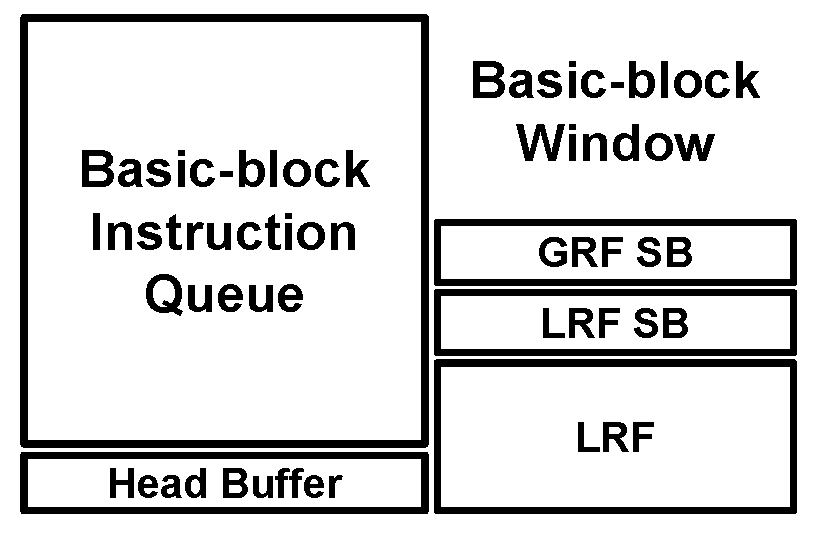
\includegraphics[width=0.6\columnwidth]{fig/bb_window.pdf} 
	\caption{Basicblock window structure}
	\label{fig:bb_window}
\end{figure}

\textbf{LRF} is a simple register file with at most 8 statically
allocated register elements. Each BB Window has its own dedicated basic-block
that is used to support storing register entries that are live only within the
basic-block lifetime. Once the basic-block completes its execution, the content
of these LRF's are invalidated. Figure~\ref{fig:bb_window} illustrates the hardware
elements supporting BB Window. GRF SB and LRF SB are the scoreboard tables used
to store the basic-block global read. A LRF SB entry is made valid once its
corresponding write operands updates the LRF. A GRF SB entry is also updated
when a global operands is about to write its valud to the GRF; the difference is a
global operand broadcasts to all GRF SB's. Since GRF SB's are small CAM arrays
with at most 7 global entries, the energy overhead of updating them is
negligible compared to an instruction window broadcast update.

Head Buffer in Figure~\ref{fig:bb_window} holds the instruction(s) pending to be
issued from the BB Window.

Figure XX shows the average number of in-flight basicblocks for SPEC2006
benchmark.

%Instructions hold offset to the instruction rather than to actual register
%address. This cuts back the register address by half (making the ISA shorter)
%    and also enable RAM lookup to the GRF table upon lookup.

%GRF scoreboard update is CAM baesd, but its lookup is RAM based. (very cheap)
%    update: CAM lookup to address ready bit
%    lookup: RAM lookup to the 1bit entry.



\subsubsection{Register File Structure}
\label{sec:reg_files}

We find that on average roughly 50\% of data communication in SPEC benchmarks
are done across def-uses that have sub-basicblock live ranges. Such registers
do not need to be register renamed if an additional register space is available
for them to temporarily hold their values for the upcoming user instruction.  As
a result, two classes of registers are defined in this architecture: local registers
and a global register. The global register is a big register file with register
renaming support. Local registers, on the other hand, are small register
file blocks with no register renaming; allocation for these registers is
done at compile time.  Global registers are designed for data communication
across basicblocks while local registers are designed for data communication
within a bsaicblock.

\subsubsection{Basicblock Reorder Buffer (BBROB)}
\label{sec:bb_rob}

Contrary to the OoO execution model where the program order is tracked at
instruction granularity through the reorder buffer (ROB), in this design, we only
track program order at basic-block granularity. BBROB is a content addressable
memory array (CAM) with only 16 entries (~10x smaller than ROB size in OoO) that
enables issuing, committing, and squashing basic-blocks as a whole in one cycle
(per basic-block). The smaller size of BBROB compared to a ROB enables
significant energy savings.

BBROB is marked complete when all its operations are completed. Complete
operands increment the completion counter in their BBROB entry. Once the counter
reaches the expected BB size, the BB is marked complete. BBE can commit up to
one BB per cycle, allowing bulk commit using one port to the table. At commit,
    the global write operands in the BB will be marked non-speculative.

%Discussion on what is held on each BBROB entry: BBID, number of completed
%basic-block instructions, total number of instructions in the BB that need to
%complete, valid bit, mis-speculation bit, global physical register writes.

%Discussion on how basic-block entry updates the GRF upon commit through its
%global physical register writes (its GRF write register(s) go from speculative
%to architectural).

%After the decode stage, a BB entry is reserved in BBROB, and when all
%instructions in a basic-block are completed and the basic-block reaches the head
%of the BBROB, the basic-block is committed as a whole in one cycle. Upon a branch
%mis-speculation event (either branch or memory), younger basic-blocks are flushed
%in one cycle. (TODO: talk more about the squash process here)


\subsection{Basicblock Scheduling}
\label{sec:scheduling}

Instruction scheduling example.

Scheduling consists of:

1) ready check: find ready instructions from head of BB - what are the
dependency checks done?

2) update check: blast write operands to all BB-header buffers. 

3) discussion of available bbWindow detection and bbWidnow allocation

% This unit is broken into two main sub-units: instruction issue and instruction
% update. The instruction issue unit looks for ready instructions at the
% head of each basicblock window buffer on every cycle. The instruction udpate
% unit updates global and local register values.
% 
% Update unit discussion goes here. It talks about updating local registers and
% their ready bits, and updating basicblock headers to indicate if the global
% operands of different instructions in a basicblock are ready.
% 
% Issue unit discussion goes here. It talks about how the issue unit checks the
% corresponding local and global operands of an instruction to determine if the
% instruction is ready. Global operands availability is checked by looking up the
% BB header (where the update unit marks a valid bit for each pgysical global
% operand that is ready) and the local operands are checked by lookup
% their up valid bit in the corresponding LRF. 
% 
% Here we also discuss the energy efficiency implications of looking up the head
% of 16 basicblock buffers rather than blasting through a 120 entry instruction
% window (which is a CAM array). We also discuss how basicblock headers help
% reduce the number of check-for-ready-operands accesses to GRF by keeping ready
% information for each global register value in the header of the BB.
% %TODO you need to implement this

\subsection{Squash Handling}
\label{sec:speculation}

In BBE, squash events are handled at basic-block granularity. To avoid wasting
{\it{useful}} instructions executed in a mis-speculated BB, the compiler uses
profiling information to separate weakly biased branches form the rest of the BB
into a single-instruction BB. Less than XX\% of useful instructions are wasted
in BBE.

The average number of BB's squashed per mis-prediction event is 6 where each
basic-block has an average of 3 global write operands. BBE is able to invalidate
register renaming entries within 5 cycles which is comparable to the number of
cycles OoO takes to restore a checkpoint and restart the execution. This
approach eliminates the need for both program checkpointing and a second
register alias table.

% how many cycles does it take to load a checkpoint?
% how much energy is it to track checkpoints?


%Memory mis-prediction is less likely in this model as each basicblock buffer
%runs in-order (no chance of mis-speculation between load-stores within a
%basicblock). We also say that mis-speculation handling is the same for
%both memory and branch.


\section{Compiler Framework}
\label{sec:compiler}

Talk about two main elements: instruction scheduling algorithm discussion (done for optimal
static schedule) and local registre allocation algorithm.

I should also talk about program profiling to find UPLD's.

\section{Simulation Framework}
\label{sec:simulation}

Discussion on the simulator parameters, use of Pintool, pinpoints, wrong-path
execution support, energy model integration.

Discussion on the benchmark

Simulator framework: pin, wrong-path, energy, speculation, function vs. timing
simulation, pin-points?

\section{Results Discussion}
\label{sec:discussion}


Figure~\ref{fig:overall} illustrates the performance, energy, and the
energy-delay (ED) product  of the OoO and BB cores normalized to the InO
processor.  On average, BB closes 70\% of the performance gap between INO and
OoO while closing 66\% of their energy gap. Overall, the energy delay product of
BB is 27\% more effective than InO and 25\% more effective than OoO.
\begin{figure*}[h]
	\centering
	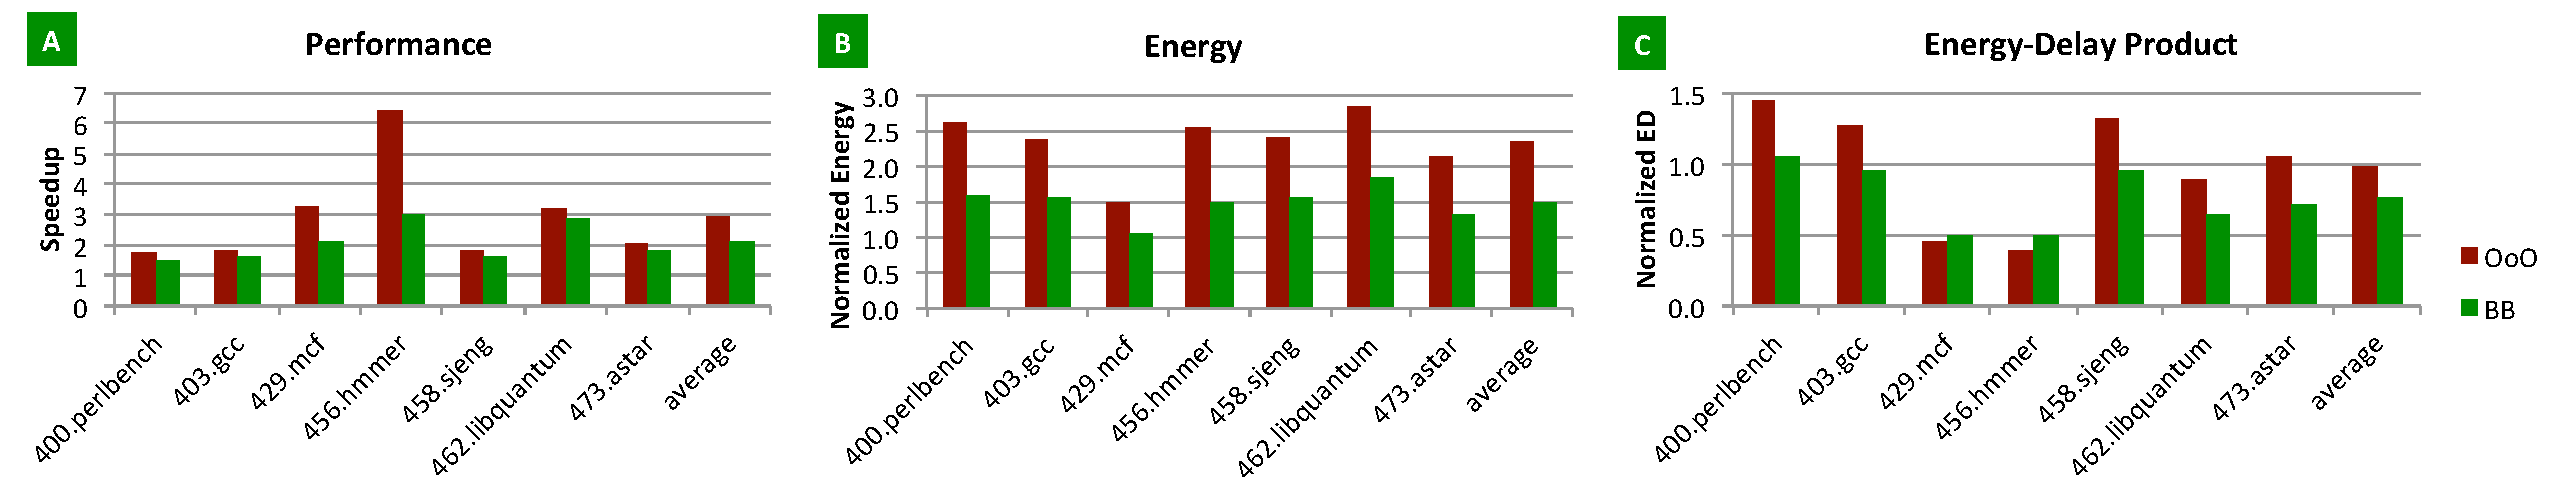
\includegraphics[width=\textwidth]{result/overall_perf.pdf} 
    \caption{(A) $IPC_{CORE}/IPC_{BASE}$, (B) $E_{CORE}/E_{BASE}$, (C)
        $ED_{CORE}/ED_{BASE}$; $CORE$ refers to BB and OoO and $BASE$ refers to
            INO core.}
	\label{fig:overall}
\end{figure*}

Figure~\ref{fig:ep} illustrates the energy versus performance plot for the three
processors when using 2-wide, 4-wide, and 8-wide architectures. Each point on
the figure is the average (speedup, energy) of SPEC benchmarks evaluated here.
While OoO provides best performance, we see the BB architecture with 8
functional units is at the lowest right corner of the graph, making it the best
design choice. Comparing Figure~\ref{fig:ep} with Figure~\ref{fig:insight} shows
the effect of the BB architecture in pushing the trend towards the more energy
efficient corner. There is still more work to be done to push the performance
point of BB further to the right.
\begin{figure}[!htbp]
	\centering
	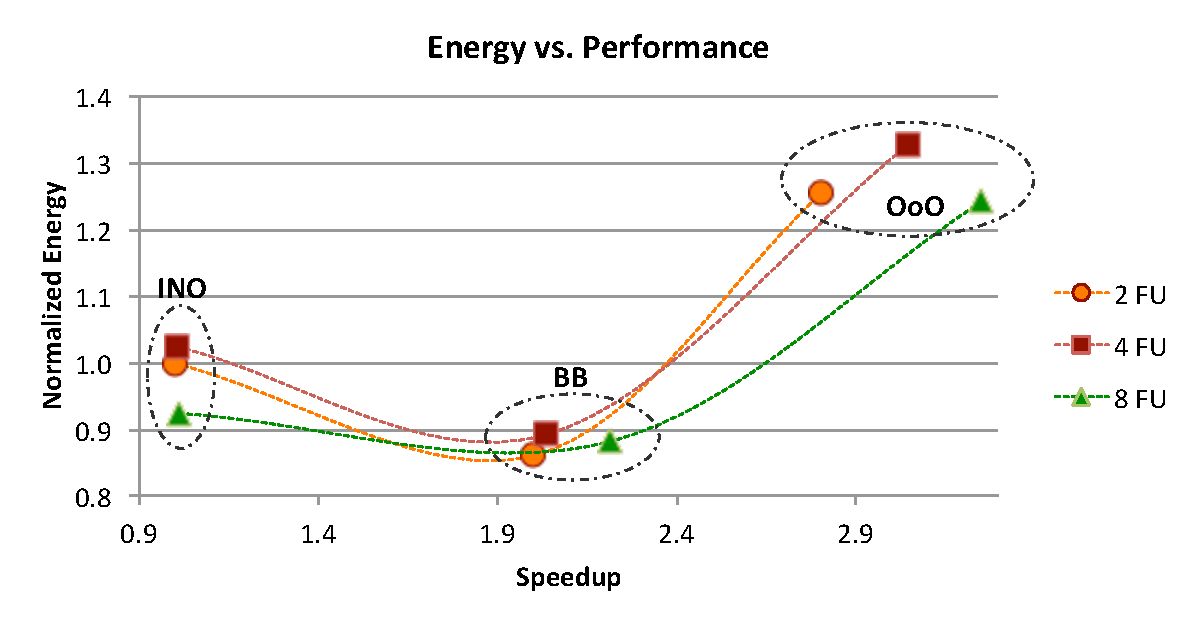
\includegraphics[width=1.0\columnwidth]{result/ep.pdf} 
    \caption{Energy vs. Performance Trend for OoO, BB, \& InO}
	\label{fig:ep}
\end{figure}

Figure~\ref{fig:bbWin_size} illustrates the change in performance and energy of
BB when the BB Window size changes. Recall that the number of available FIFO
slots in these buffers define how the compiler partitions basic-blocks. The
smaller the FIFO size, the more fine grain the code, the more the number of BB's
in-flight to issue instructions. Overall, we observe 15\% average performance
drop and XX\% energy gain when BB Window size changes from 5 to 15 entries.
\begin{figure}[!htbp]
	\centering
	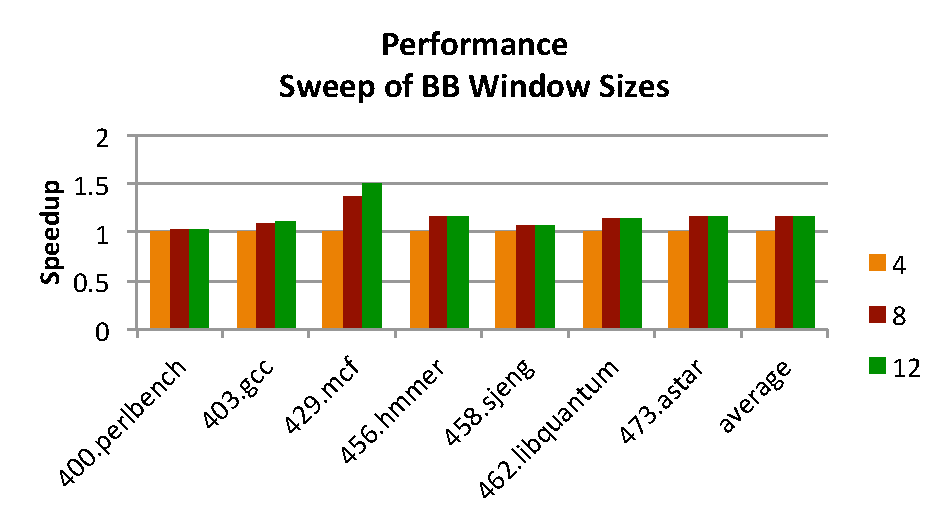
\includegraphics[width=1.0\columnwidth]{result/bbWin_size.pdf} 
    \caption{Performance \& energy change with sweeping the BB Window FIFO queue size}
	\label{fig:bbWin_size}
\end{figure}

Figure~\ref{fig:bbWin_ins_cnt} evaluates the effect of BB Window count on the
performance of BB architectures. We observe 16\% speedup gain between 4 and 8
instruction BB Windows, but not so much beyond. This result suggests  eight BB
Windows are sufficient to get optimum performance gains while keeping the energy
at a relatively low value. Because gcc has small basic-blocks with independent
instructions, it makes best use of the extra BB Window resources to improve the
ILP by up to 50\% while saving up to 8\% in energy as a result.
\begin{figure}[!htbp]
	\centering
	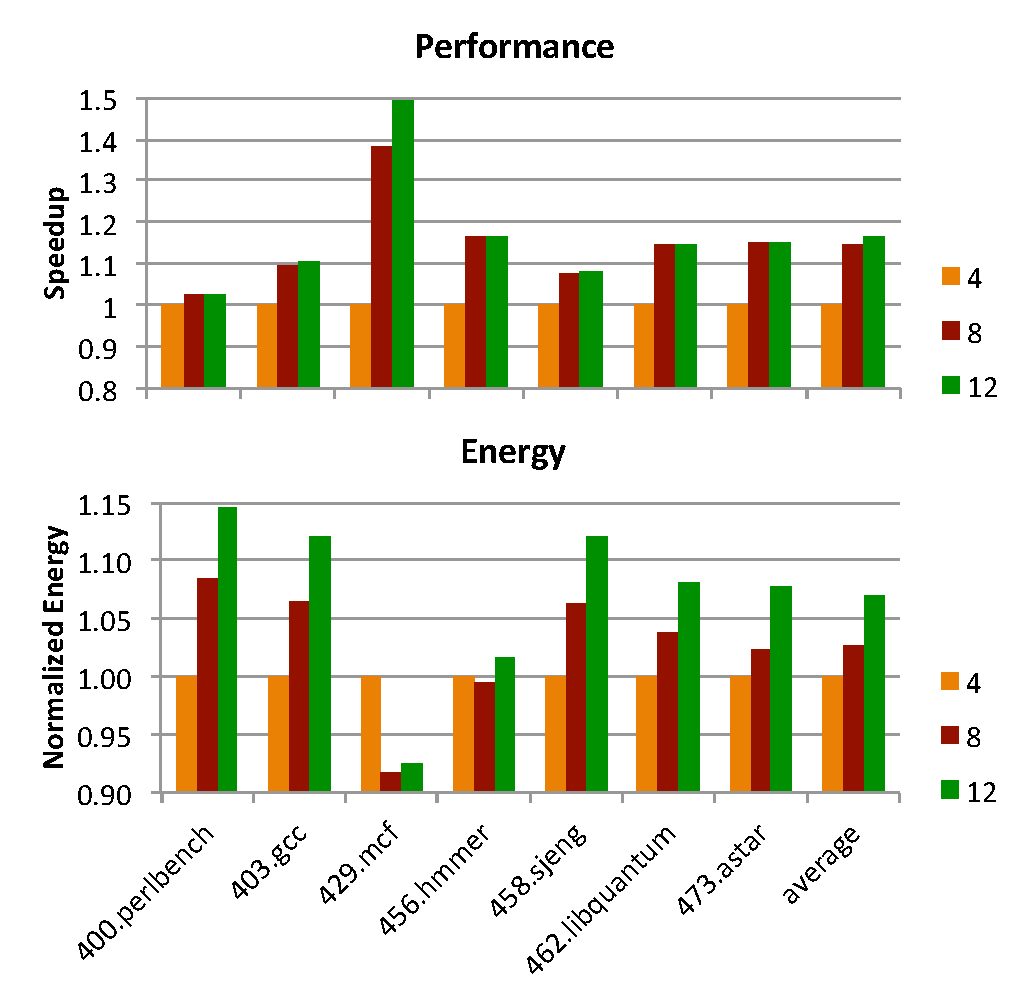
\includegraphics[width=1.0\columnwidth]{result/bbWin_ins_cnt.pdf} 
    \caption{Performance \& energy change with sweeping the number of BB Windows}
	\label{fig:bbWin_ins_cnt}
\end{figure}

Figure~\ref{fig:bbWin_port} evaluates the performance improvement trend as the
number of read ports for BB Windows increase from 1 to 8 ports. While eight
ports provides 11\% average performance gains, three ports provides 10\%.  Given
the XX\% energy overhead of 8-ported BBWindows, we find three read ports the
optimal port count for achieving optimal ED product.
\begin{figure}[!htbp]
	\centering
	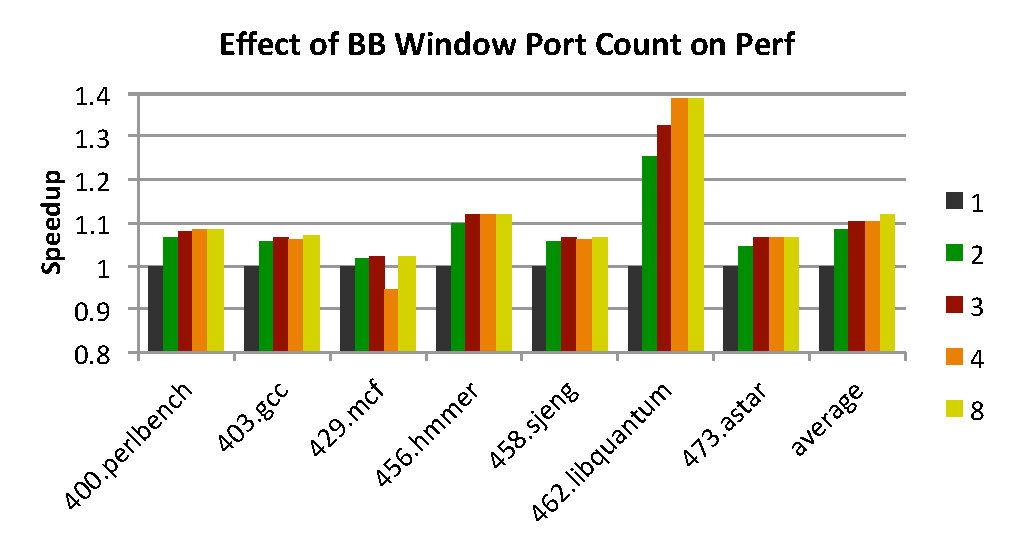
\includegraphics[width=1.0\columnwidth]{result/bbWin_port.pdf} 
    \caption{Performance \& energy change with sweeping the number of BB Window
    ports}
	\label{fig:bbWin_port}
\end{figure}

Figure~\ref{fig:lrf_effect} shows 12\% average increase in speedup and 19\%
reduction in energy consumption of BBE when the register allocator uses LRF
versus when it only uses the global register file for all operations.
\begin{figure}[!htbp]
	\centering
	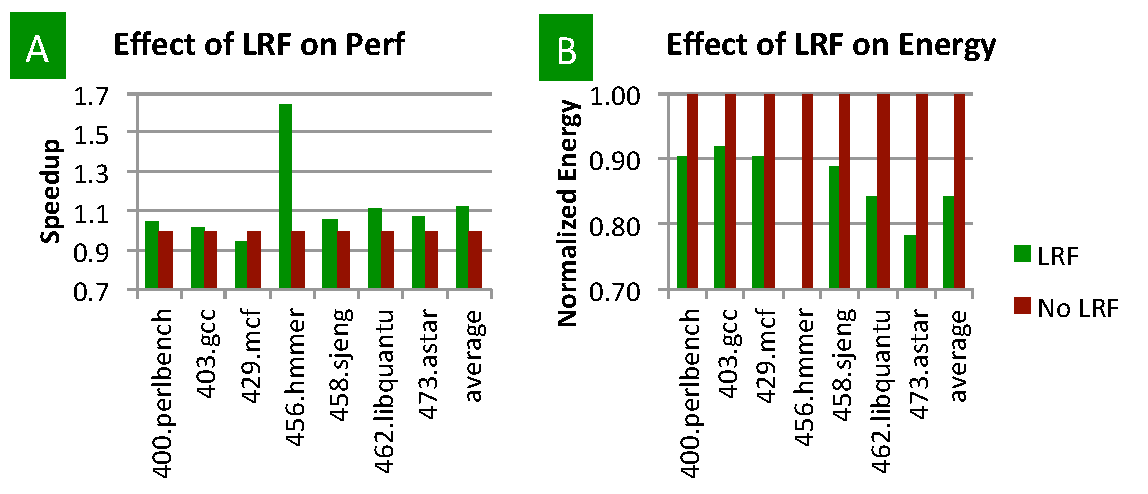
\includegraphics[width=1.0\columnwidth]{result/lrf_effect.pdf} 
    \caption{Performance \& energy change with sweeping the number of BB Windows}
	\label{fig:lrf_effect}
\end{figure}


As mentioned earlier in the paper, BBE benefits from optimal basic-block
instructions scheduling, making each basic-block issue instructions at the
highest issue rate possible. This implies enabling the scheduler to identify
data dependency chains in the code and scheduling instructions such that they
can be issued back-to-back while using the common data-bus for reading their
input operands. Figure~\ref{fig:forwarding} shows BB is 39\% more effective in
leveraging data-forwarding while issuing instructions. The bar charts are
normalize to the forwarding ability of the InO core. 
\begin{figure}[!htbp]
	\centering
	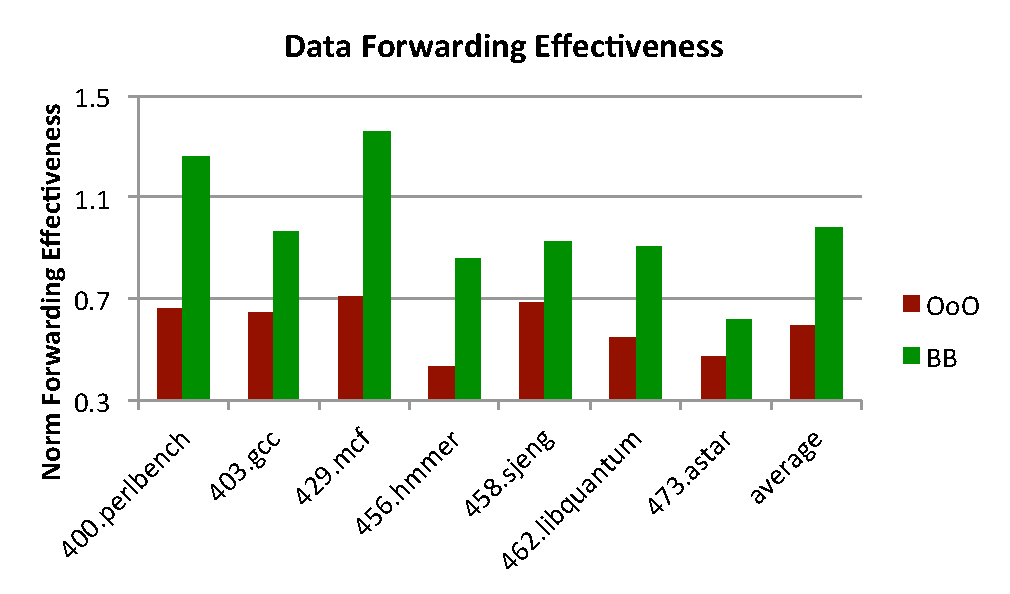
\includegraphics[width=1.0\columnwidth]{result/forwarding.pdf} 
    \caption{Energy vs. Performance Trend for OoO, BB, \& InO}
	\label{fig:forwarding}
\end{figure}

As mentioned in Section~\ref{sec:bpu}, the BB core reduces the number branch
lookup accesses to the branch prediction unit, including the BTB.
Figure~\ref{fig:bpu} illustrates, on average, BB looks up the BPU 35\% less
frequently, making it just as much more energy efficient than OoO.
\begin{figure}[!htbp]
	\centering
	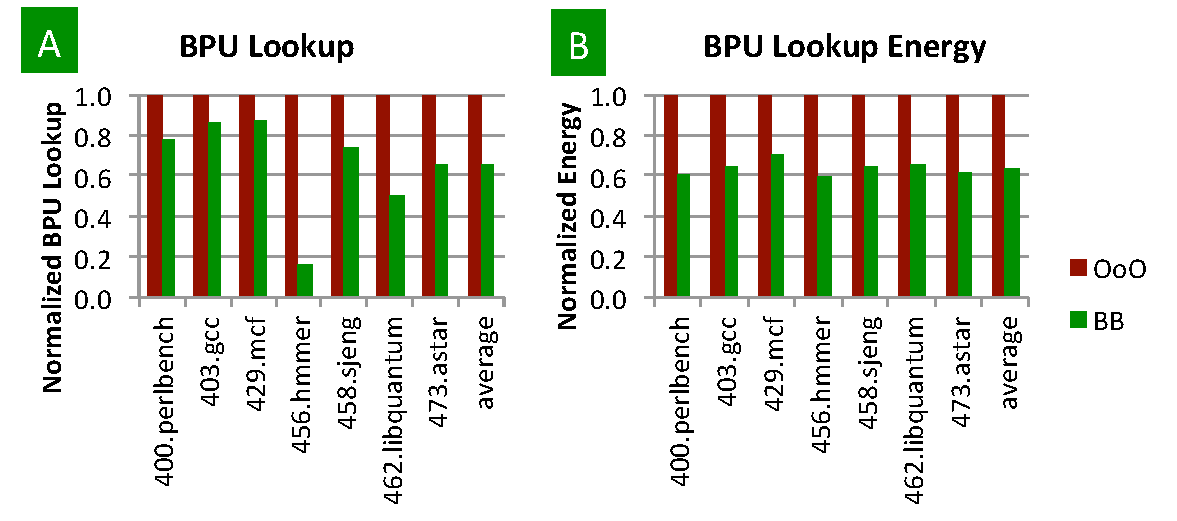
\includegraphics[width=1.0\columnwidth]{result/bpu.pdf} 
    \caption{(A) Normalized ratio of BPU accesses by BBE wrt. OoO. (B)
        Normalized lookup energy reduction ratio of BB wrt. OoO.}
	\label{fig:bpu}
\end{figure}


area evaluation.

energy breakdown pie chart

%evaluation of pipeline stages.
%comparison of new and conventional register rename model.
%comparison of new and conventional squash mode.
%sweep of register file sizes. 



%\section{outline}
\label{sec:outline}

In this paper I would like to point out the following achievements we have
made:

\begin{itemize} 
    \item energy efficient and high performance computing need for dynamism and
speculation (INTRO)
    \item compiler design
    \item architecture design
    \item pipeline energy efficiency opportunities
    \item ?
    \item results
    \item recovery time, energy, performance, register file behavior, LSQ,
wakeup logic information, having multiple issue elements from each BB
    \item simulation framework
    \item discussion
\end{itemize}


%%%%%%% CITATIONS %%%%%%%
\bstctlcite{bstctl:etal, bstctl:nodash, bstctl:simpurl}
\bibliographystyle{IEEEtranS}
\bibliography{references}

\end{document}

